\chapter{Function Transformations}

Write the function for $g(x)$ if it is the result of $f(x)$ after the following ordered sequence of transformations.
\begin{enumerate}
\item \begin{enumerate}[(1)]
	\item Vertical stretch by 3
	\item Shift left 1 unit
	\item Reflect across $y$-axis
\end{enumerate}
\item \begin{enumerate}[(1)]
	\item Horizontal compression by 2
	\item Shift up 1 unit
\end{enumerate}
\item \begin{enumerate}[(1)]
	\item Reflect across $x$-axis
	\item Vertical compression by 4
	\item Move right 7 units
\end{enumerate}
\setcounter{Review}{\value{enumi}}
\end{enumerate}

Write the function $g(x)$ that is a result of the following ordered sequence of transformations to $f(x)=|x|$.
\begin{enumerate}
\setcounter{enumi}{\value{Review}}
\item
\begin{enumerate}[(1)]
\item Reflect across $x$-axis
\item Shift right 3 units
\item Horizontal stretch by factor of 5
\end{enumerate}

\item
\begin{enumerate}[(1)]
\item Shift down 2 units
\item Reflect across $y$-axis
\item Shift up 1 unit
\end{enumerate}

\item
\begin{enumerate}[(1)]
\item Horizontal compression by factor of 7
\item Vertical compression by factor of 4
\item Shift left 9 units
\end{enumerate}
\setcounter{Review}{\value{enumi}}
\end{enumerate}

Given $f(x) = \sqrt{x}$, determine the resulting function $g(x)$ after the following ordered sequence of transformations.
\begin{enumerate}
\setcounter{enumi}{\value{Review}}
\item
\begin{enumerate}[(1)]
\item Shift up 2 units
\item Horizontal stretch by 5
\item Shift left 3 units
\end{enumerate}

\item
\begin{enumerate}[(1)]
\item Vertical compression by factor of 3
\item Reflect across $y$-axis
\item Horizontal compression by 5
\end{enumerate}

\item
\begin{enumerate}[(1)]
\item Shift right 8 units
\item Reflect across $x$-axis
\item Horizontal compression by factor of 4
\end{enumerate}
\setcounter{Review}{\value{enumi}}
\end{enumerate}

\newpage

Write the final equation of $g(x)$ if it is found by taking $f(x) = \sqrt{x}$ after the following ordered sequence of transformations.   

\begin{enumerate}	\setcounter{enumi}{\value{Review}}
\item \begin{enumerate}[(1)]
\setlength\itemsep{0pt}
    \item Shift right 2 units
    \item Horizontal stretch by factor 3
    \item Shift down 2 units
    \item Reflect across $x$-axis
\end{enumerate}

\item
\begin{enumerate}[(1)]
\setlength\itemsep{0pt}
    \item Horizontal stretch by factor 3
    \item Shift left 1 unit
    \item Shift up 2 units
    \item Reflect across $y$-axis
\end{enumerate}

\item
\begin{enumerate}[(1)]
\setlength\itemsep{0pt}
    \item Vertical stretch by factor 5
    \item Horizontal stretch by factor 2
    \item Shift up 3 units
    \item Reflect across $x$-axis
\end{enumerate}
\setcounter{Review}{\value{enumi}}
\end{enumerate}

Find the equation for $g(x)$ if $g(x)$ is found by performing the following \emph{ordered} sequence of transformations to $f(x)=\frac{1}{x}$.

\begin{enumerate}	\setcounter{enumi}{\value{Review}}
\item \begin{enumerate}[(1)]
\setlength\itemsep{0pt}
	\item Shift left 3 spaces
	\item Reflect across $y$-axis
	\item Shift down 5 spaces
	\item Vertical stretch by factor of 7
\end{enumerate}
\setcounter{Review}{\value{enumi}}
\end{enumerate}

\begin{enumerate}	\setcounter{enumi}{\value{Review}}
\item \begin{enumerate}[(1)]
\setlength\itemsep{0pt}
	\item Shift up 3 spaces
	\item Reflect across $x$-axis
	\item Shift right 5 spaces
	\item Horizontal compression by factor of 7
\end{enumerate}
\setcounter{Review}{\value{enumi}}
\end{enumerate}

Given $f(x) = x^3$, determine the equation for $g(x)$ after the following \emph{ordered} sequence of transformations to $f(x)$.
\begin{enumerate}	\setcounter{enumi}{\value{Review}}
\item \begin{enumerate}[(1)]
\setlength\itemsep{0pt}
	\item Vertical stretch by factor of 4
	\item Shift up 3 units
	\item Reflect across $y$-axis
	\item Shift down 5 units
\end{enumerate}
\setcounter{Review}{\value{enumi}}
\end{enumerate}

\begin{enumerate}	\setcounter{enumi}{\value{Review}}
\item \begin{enumerate}[(1)]
\setlength\itemsep{0pt}
	\item Horizontal compression by factor of 3
	\item Shift right 4 units
	\item Shift up 1 unit
\end{enumerate}
\setcounter{Review}{\value{enumi}}
\end{enumerate}

\begin{enumerate}	\setcounter{enumi}{\value{Review}}
\item \begin{enumerate}[(1)]
\setlength\itemsep{0pt}
	\item Reflect across $x$-axis
	\item Shift down 5 units
	\item Vertical compression by factor of 5
	\item Horizontal stretch by factor of 9
\end{enumerate}
\setcounter{Review}{\value{enumi}}
\end{enumerate}

Given the graph of $f(x)$ below, find the new coordinates of each point after the following transformations.
\begin{center}
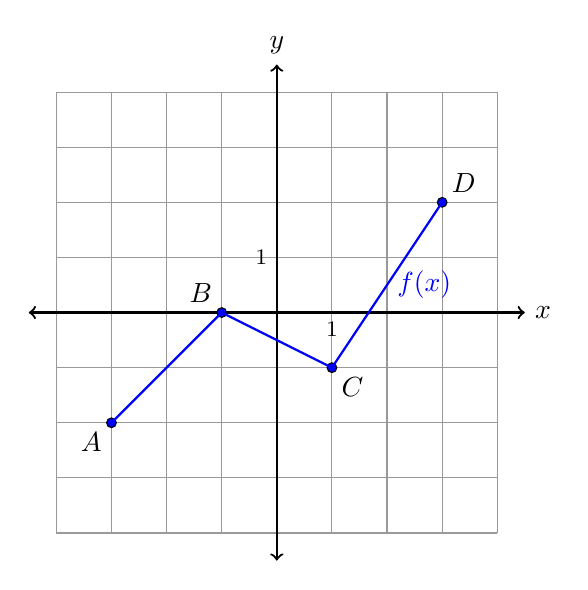
\begin{tikzpicture}[scale=0.7]
\draw[gray!80] (-4,-4) grid (4,4);
\draw[<->, thick] (-4.5,0) -- (4.5,0) node [right] {$x$};
\draw[<->, thick] (0,-4.5) -- (0,4.5) node [above] {$y$};
\coordinate (A) at (-3,-2);
\coordinate (B) at (-1,0);
\coordinate (C) at (1,-1);
\coordinate (D) at (3,2);
\draw[fill=blue] (A) circle [radius=2.5pt] node [below left] {$A$};
\draw[fill=blue] (B) circle [radius=2.5pt] node [above left] {$B$};
\draw[fill=blue] (C) circle [radius=2.5pt] node [below right] {$C$};
\draw[fill=blue] (D) circle [radius=2.5pt] node [above right] {$D$};
\draw[thick,blue] (A) -- (B) -- (C) -- node [midway, right] {$f(x)$} (D);
\node at (1,0) [below] {\footnotesize 1};
\node at (0,1) [left] {\footnotesize 1};
\end{tikzpicture}
\end{center}

\begin{multicols}{3}
\begin{enumerate} \setcounter{enumi}{\value{Review}}
    \item $-2f(x+1)$ 
    \item $f\left(-\frac{1}{2}x\right)-3$
    \item $\frac{1}{2}f(-x-2)+2$
\end{enumerate}	\setcounter{Review}{\value{enumi}}
\end{multicols}
\begin{multicols}{3}
\begin{enumerate}	\setcounter{enumi}{\value{Review}} 
    \item $f(2x+2)-1$
    \item $-3f(-x+1)+2$
    \item $5f\left(-\frac{1}{2}x\right)$
\setcounter{Review}{\value{enumi}}
\end{enumerate}
\end{multicols}

Given $f(x)$ below, determine the coordinates of $A'$, $B'$, $C'$, and $D'$ after the final transformations done to $f$.
\begin{center}
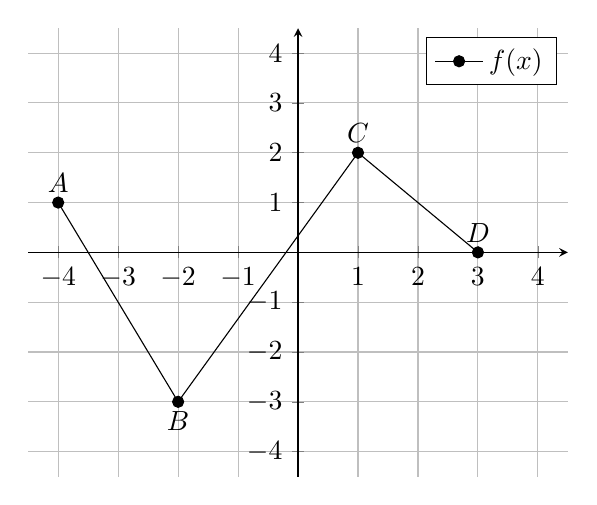
\begin{tikzpicture}
\begin{axis}[
axis lines = middle, xmin = -4.5, xmax = 4.5, xtick distance = 1, ymin = -4.5, ymax = 4.5, ytick distance = 1, grid]
\addplot [mark = *] coordinates {
(-4,1) (-2,-3) (1,2) (3,0)
};
\addlegendentry{$f(x)$};
\node at (-4,1) [above] {$A$};
\node at (-2,-3) [below] {$B$};
\node at (1,2) [above] {$C$};
\node at (3,0) [above] {$D$};
\end{axis}
\end{tikzpicture}
\end{center}
\begin{multicols}{4}
\begin{enumerate}	\setcounter{enumi}{\value{Review}} 
\item $f(-2x-5)+4$
\item $\frac{1}{3}f(x+4)-1$
\item $-3f\left(-\frac{1}{2}x-3\right)$
\item $f(4x+3)+8$
\end{enumerate}	\setcounter{Review}{\value{enumi}}
\end{multicols}



\newpage

\section{Answer Key}

\begin{enumerate}
	\item $g(x) = 3f(-x+1)$
	\item $g(x) = f(2x)+1$
	\item $g(x) = -\frac{1}{4}f(x-7)$
    \item $g(x) = -\left|\frac{1}{5}x-3\right|$
    \item $g(x) = |-x|-1$
    \item $g(x) = \frac{1}{4}|7(x+9)| = \frac{1}{4}|7x+63|$
    \item $g(x) = \sqrt{\frac{1}{5}(x+3)} + 2 = \sqrt{\frac{1}{5}x + \frac{3}{5}}+2$
    \item $g(x) = \frac{1}{3}\sqrt{-5x}$
    \item $g(x) = -\sqrt{4x-8}$
    \item $g(x) = -\left(\sqrt{\frac{1}{3}x-2}-2\right) = -\sqrt{\frac{1}{3}x-2}+2$
    \item $g(x) = \sqrt{\frac{1}{3}(-x+1)}+2 = \sqrt{-\frac{1}{3}x+\frac{1}{3}}+2$
    \item $g(x) = -\left(5\sqrt{\frac{1}{2}x}+3\right) = -5\sqrt{\frac{1}{2}x} - 3$
    \item $g(x) = \frac{7}{-x+3} - 35$
    \item $g(x) = -\frac{1}{7x-5} - 3$ 
    \item $g(x) = 4(-x)^3 - 2$
    \item $g(x) = \left(3(x-4)\right)^3 + 1$
    \item $g(x) = \frac{1}{5}\left(-\frac{1}{9}x\right)^3 - 5$
    \item $A'(-4,4), \, B'(-2,0), \, C'(0,2), \, D'(2,-4)$
    \item $A'(6,-5), \, B'(2,-3), \, C'(-2, -4), \, D'(-6,-1)$
    \item $A'(1,1), \, B'(-1,2), \, C'(-3,1.5), \, D'(-5,3)$
    \item $A'(-2.5,-3), \, B'(-1.5,-1), \, C'(-0.5,-2), \, D'(0.5,1)$
    \item $A'(4,8), \, B'(2,2), \, C'(0,5), \, D'(-2,-4)$
    \item $A'(6,-10), \, B'(2,0), \, C'(-2,-5), \, D'(-6,10)$
    \item $A'\left(-\frac{1}{2},5\right), \, B'\left(-\frac{3}{2},1\right), \, C'(-3,6), \, D'(-4,4)$
	\item $A'\left(-8,-\frac{2}{3}\right), \, B'(-6,-2), \, C'\left(-3,-\frac{1}{3}\right), \, D'(-1,-1)$
	\item $A'(2,-3), \, B'(-2,9), \, C'(-8,-6), \, D'(-12,0)$
	\item $A'\left(-\frac{7}{4},9\right), \, B'\left(-\frac{5}{4},5\right), \, C'\left(-\frac{1}{2},10\right), \, D'(0,8)$
\end{enumerate}
